\label{tag:experiment}
本研究ではLTIを用いることで実際に複数のLMSから、独立したWebアプリケーションであるネットワーク自己学習機能を同じように学習支援ツールとして呼び出すことができるのかを確認するために、LTIに準拠したLMSであるMoodle、Canvasを用いての実装実験を行った。\\

\subsection{LTI使用方法}
LMS上でツールプロバイダを使用するには、各LMS上で外部ツールの設定を変更する必要がある。例として、Moodleでの使用方法を説明する。\\
moodleでは外部ツール設定より図\ref{fig:moodle config}参照、ツール名、ツールURL、コンシューマキー、秘密鍵の設定をする必要がある。これらの設定を得て、moodleからツールプロパイダを利用することが可能となる。\\
\begin{figure}[htbp]
  \begin{center}
    \resizebox{\textwidth}{!}{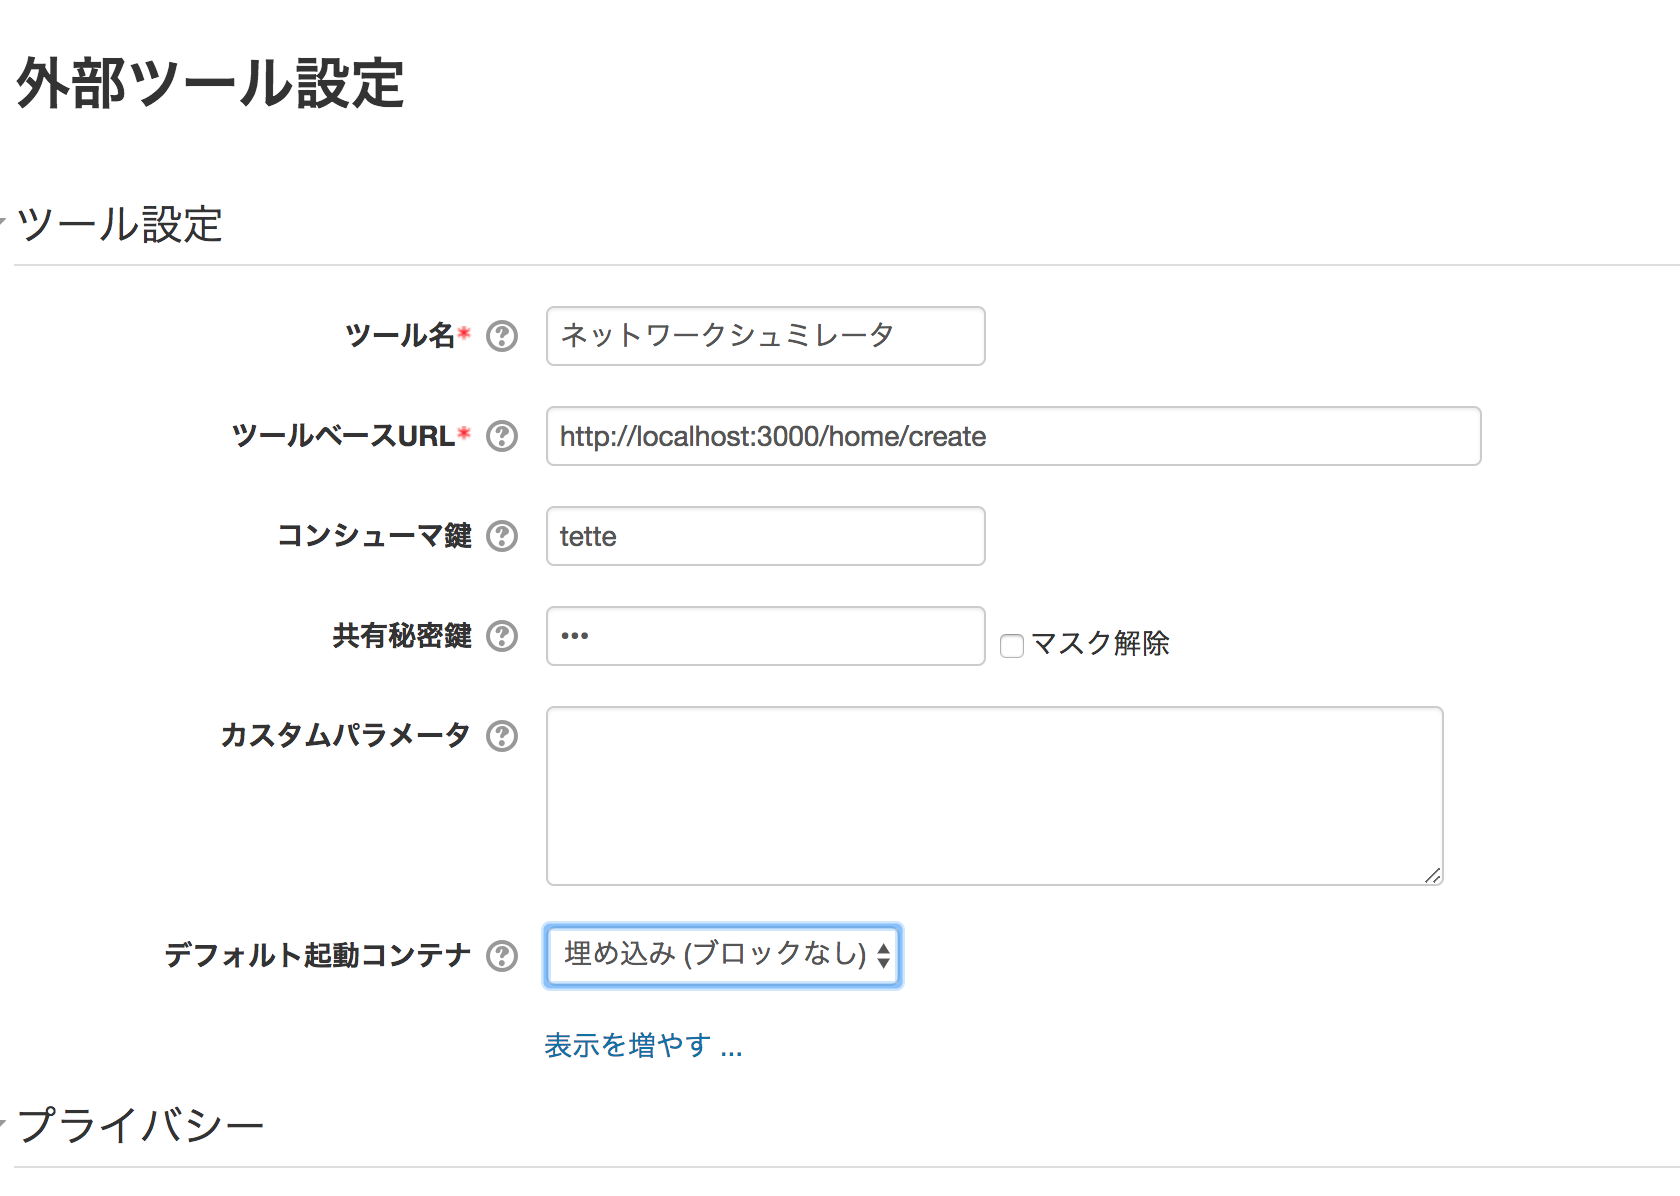
\includegraphics{img/moodleSet.png}}
    \caption{moodle 外部ツール設定画面}
    \label{fig:moodle config}
  \end{center}
\end{figure}

\subsection{外部ツールの起動}
Moodle,Canvasでの外部ツール起動画面を図\ref{fig:moodle kidou}、図\ref{fig:canvas kidou}に示す。

\begin{figure}[htbp]
  \begin{center}
    \resizebox{\textwidth}{!}{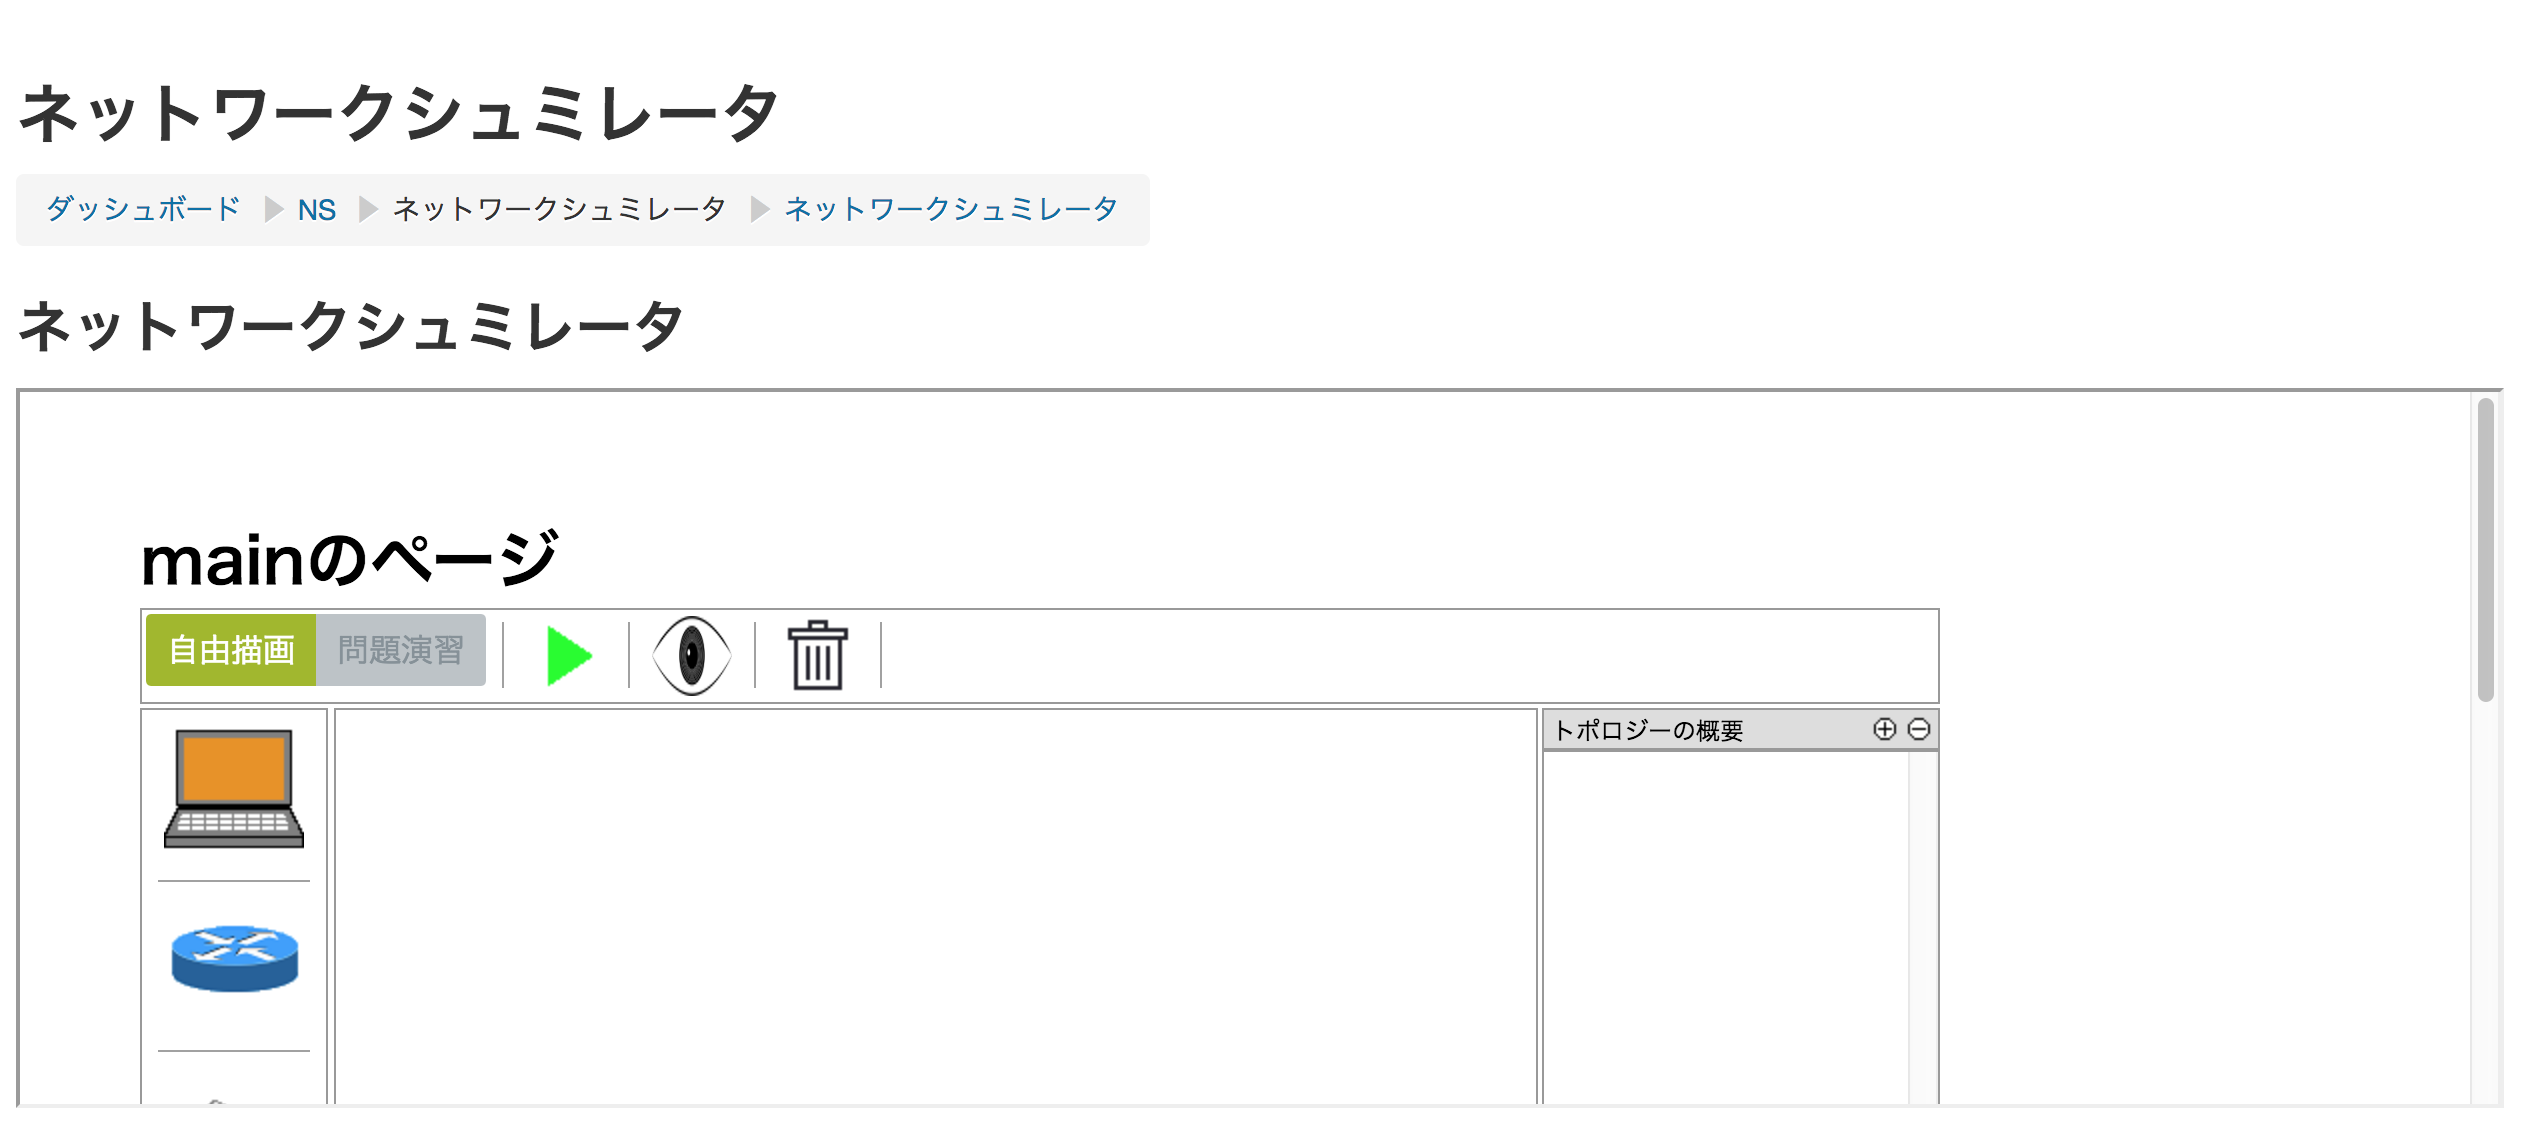
\includegraphics{img/LTIstart.png}}
    \caption{Moodle 外部ツール起動}
    \label{fig:moodle kidou}
  \end{center}
\end{figure}

\begin{figure}[htbp]
  \begin{center}
    \resizebox{\textwidth}{!}{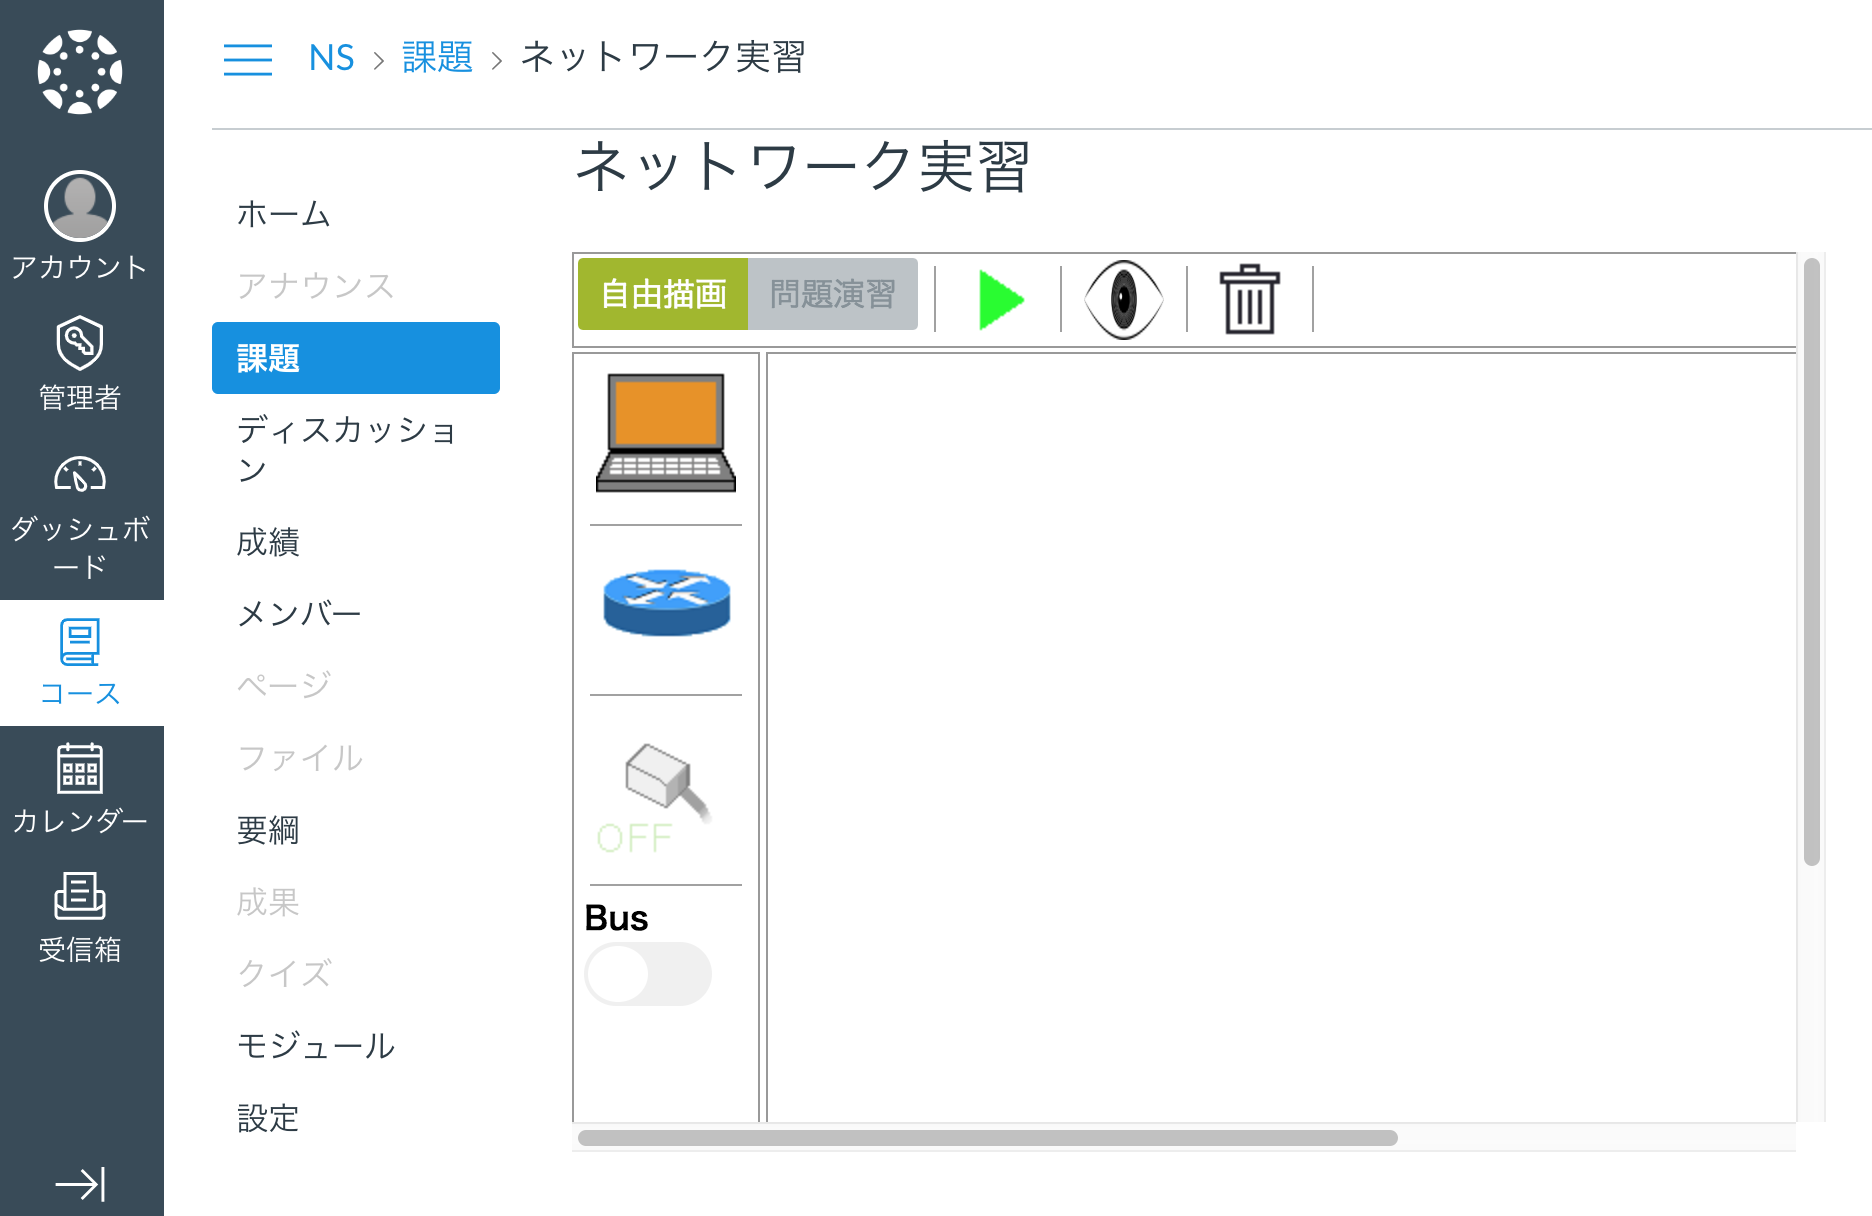
\includegraphics{img/Canvas.png}}
    \caption{Canvas 外部ツール起動}
    \label{fig:canvas kidou}
  \end{center}
\end{figure}

\subsection{成績反映に使うデータ}
実際に送信するXLMを図\ref{fig:XML}に示し、使用する値についての解説をする。\\
ユーザーを識別するための番号は「sourcedId」タグを使用。ツールコンシューマからユーザーIDが送信されるので、「sourcedId」タグ内に書き換えて、送信する。
成績データに関しては「textString」タグを使用。0.0〜1.0までの範囲で得点を操作でき、1.0で100点となる。成績反映に関してはこの二つのデータを使用することで成績を反映させた。

\begin{figure}[htbp]
  \begin{center}
    \resizebox{8cm}{!}{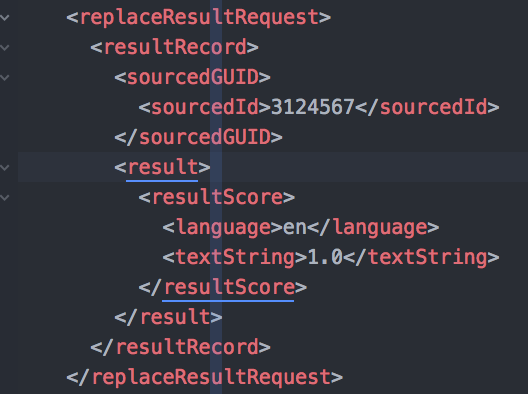
\includegraphics{img/XML.png}}
    \caption{実際に送るXML}
    \label{fig:XML}
  \end{center}
\end{figure}

\subsection{成績反映}
MoodleとCanvasにおいて、実際に成績反映の実験を行った。\\
Moodleでの成績反映は成功したが、Canvasでの成績反映はできなかった。
Moodleでの成績反映画面を図\ref{fig:moodle score}に示す。


\begin{figure}[htbp]
  \begin{center}
    \resizebox{\textwidth}{!}{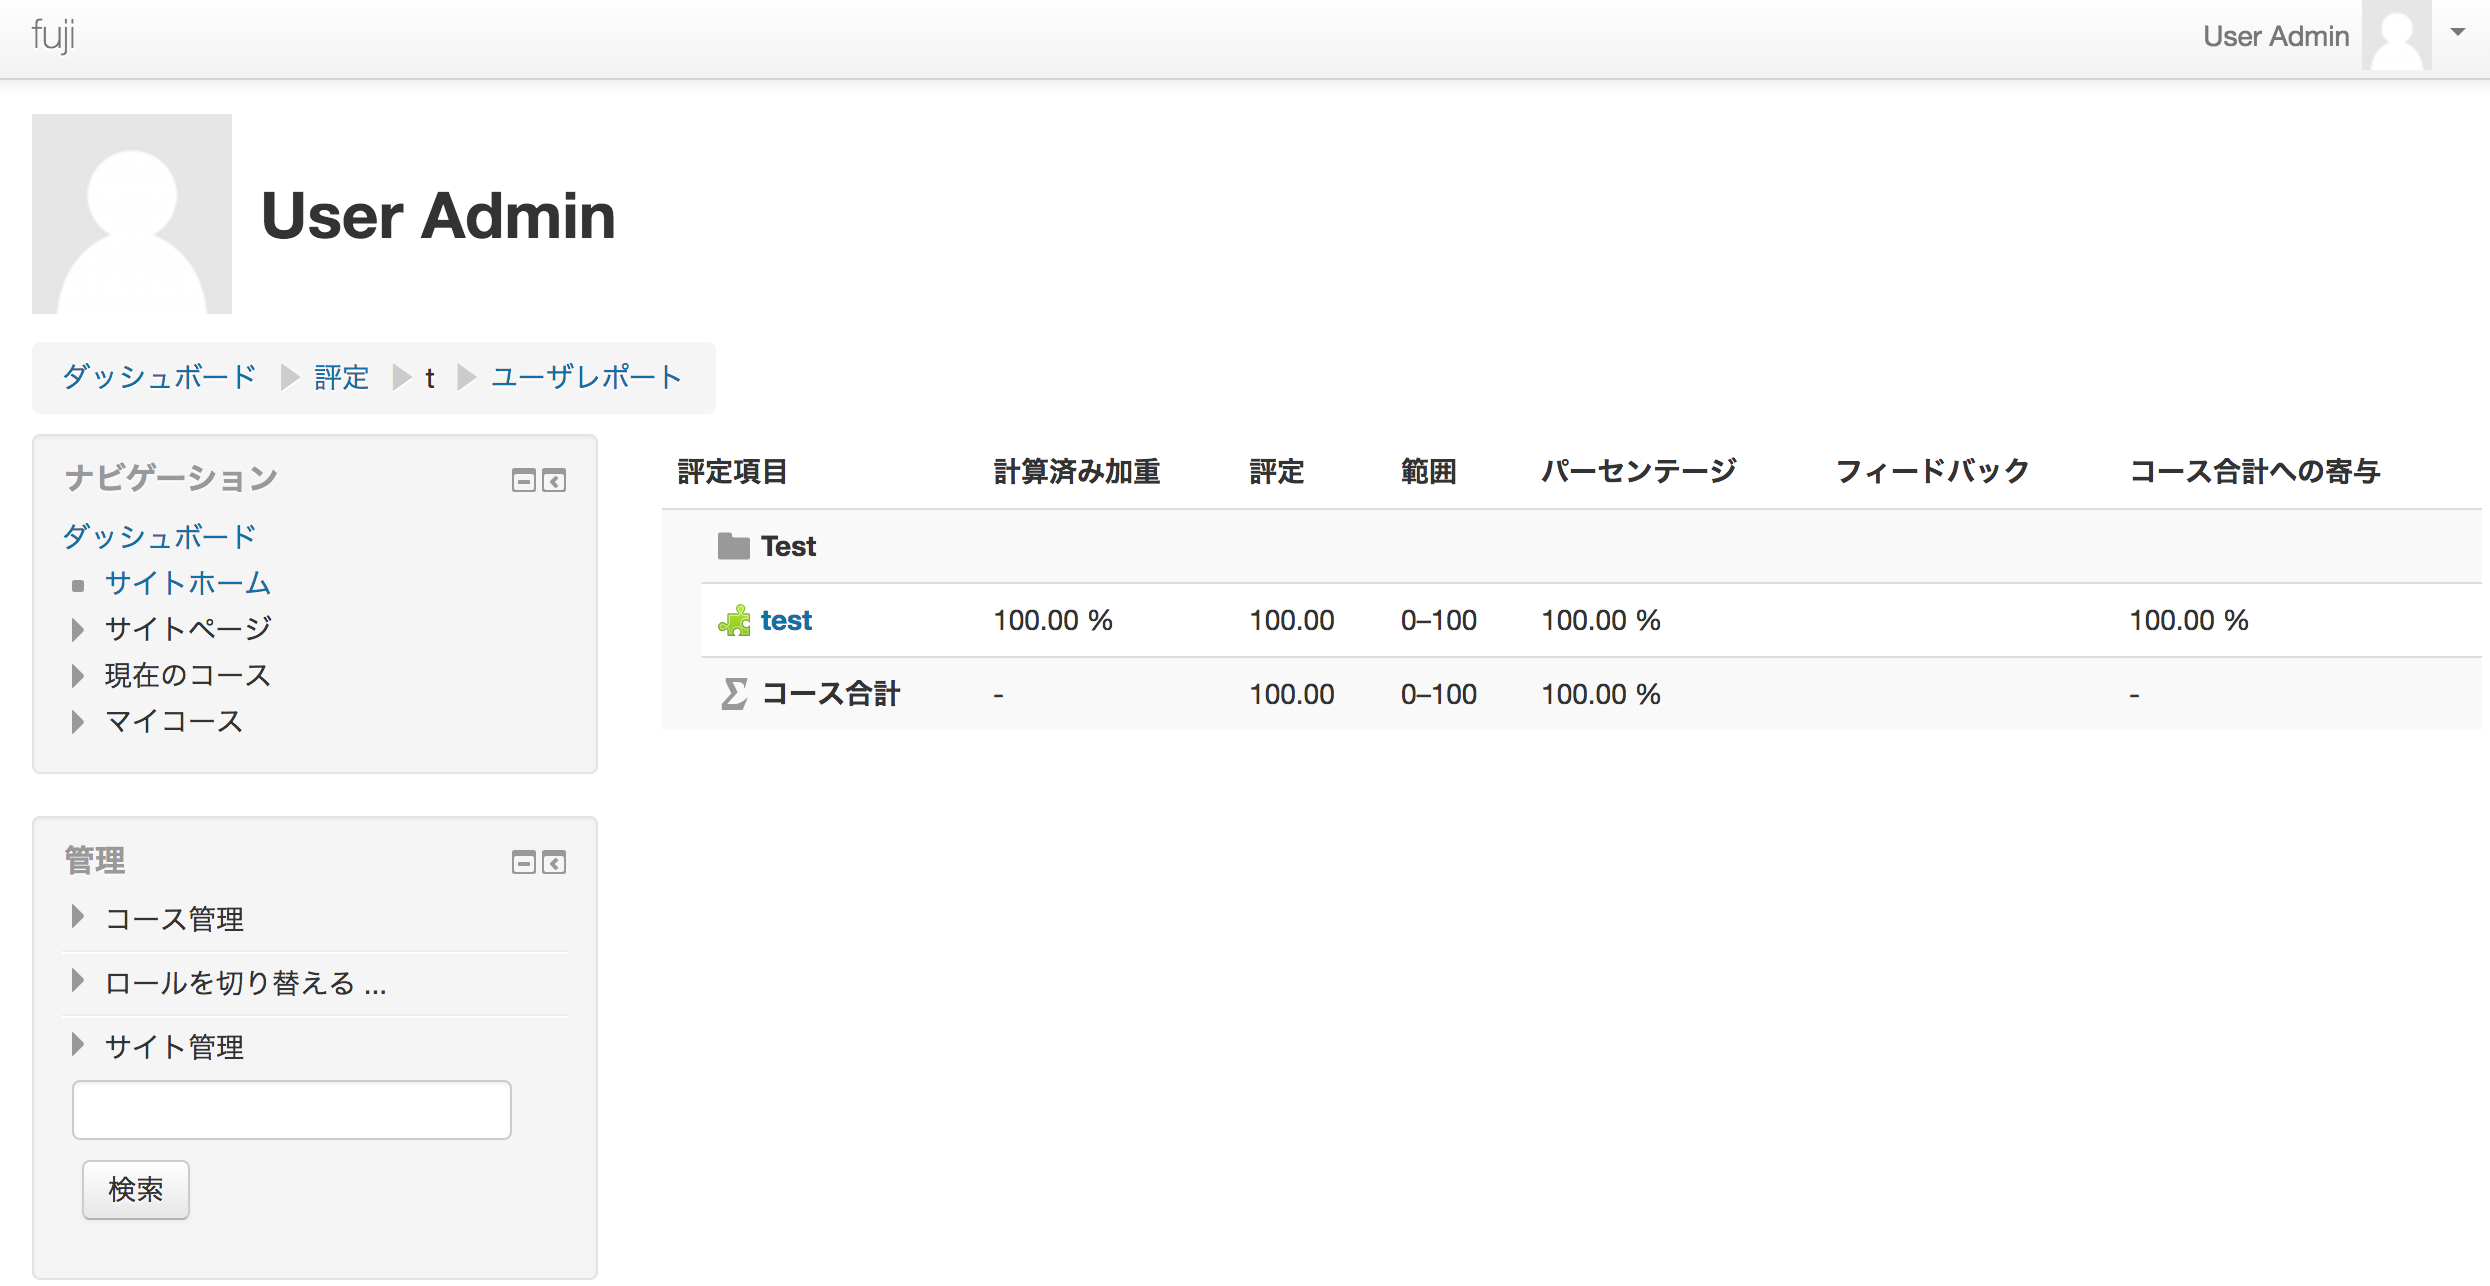
\includegraphics{img/score.png}}
    \caption{moodle 成績反映}
    \label{fig:moodle score}
  \end{center}
\end{figure}
